\chapter{Filesystem Metaphore and the Pipe Abstraction}
From our experience with building applications, there are a clear set of requirements that are necessary.  Most applications
construct the notion of context using the naming convention ascribed to a sensor stream.  The name conflates the notion of system,
space, and type information.  At the very least, these three should be supported, however, often other categorical needs must be
met to perform various kinds of aggregate statistical, analytics, and control.  In addition, we need to support the management of
processing jobs that process stream data and provide integrated management facilities for them.

Building applications are essentially monitoring and control applications built on the streams generated by sensors embedded through
the building or distillates of them.  As the number of applications and streams increased, it becomes desireable to manage them 
in a centralized fashion.  Moreover, the centralized apporach allows all applications to make use of a uniform naming convention and
can allow applications to be interoperable.  Systems that wish to support such applications require the following properties:

\begin{enumerate}
\item Logically accessible physical resources.
\item Representation of data producing and data consuming elements.
\item Representation of inter-relationships between elements.
\item Provide uniform naming and access.
\end{enumerate}

This chapter describes the use of the filesystem and pipe abstraction for represents streams in space.  The filesystem naming convention
provide a a unified namespace to application, for accessing physical resources and streams.  Moreoever, we support multi-naming through
symbolic links -- an important requirement for building applications.  We also discuss the incorporation of a pipe-like mechanism for 
processing streams and their output.


\section{Related Work}
HomeOs~\ref{homeos}


\section{File abstraction and Supporting Multiple Names}
Similar requirements to those aforementioned have been addressed in the design and implementation of filesystems.  Filesystems provide
logical access to physical resources through files, with different files and associated semantics, exposed to applications through a shell
or programmtically.  Filesystems representat collections of bits, encapsulated by a file, and grouped with folders.  Symbolic links support
the notion of multi-naming.  A single file or folder could have multiple names that lead to the same underlying object.  Filesystems even
support the notion of streaming data through character and block device files.  Moreover, pipe files allow programs to communite with each
other through a piece of shared memory, where the source application writes to the pipe and the sink application consumes from the pipe.

We assert that these constructs should be directly adopted for supporting applications in the buildings.  Our approach adopts the unix
file philosophy where everthing is represented as a file.  Each object created in StreamFS is assigned two names, by default, one which 
uniquely identifies the object and \emph{not} human-readable and the second which is changeable and human-readable.  Consider
the example shown in Figure~\cite{fig:everythingfile}.


\begin{figure}[t!] %htbp
\centering
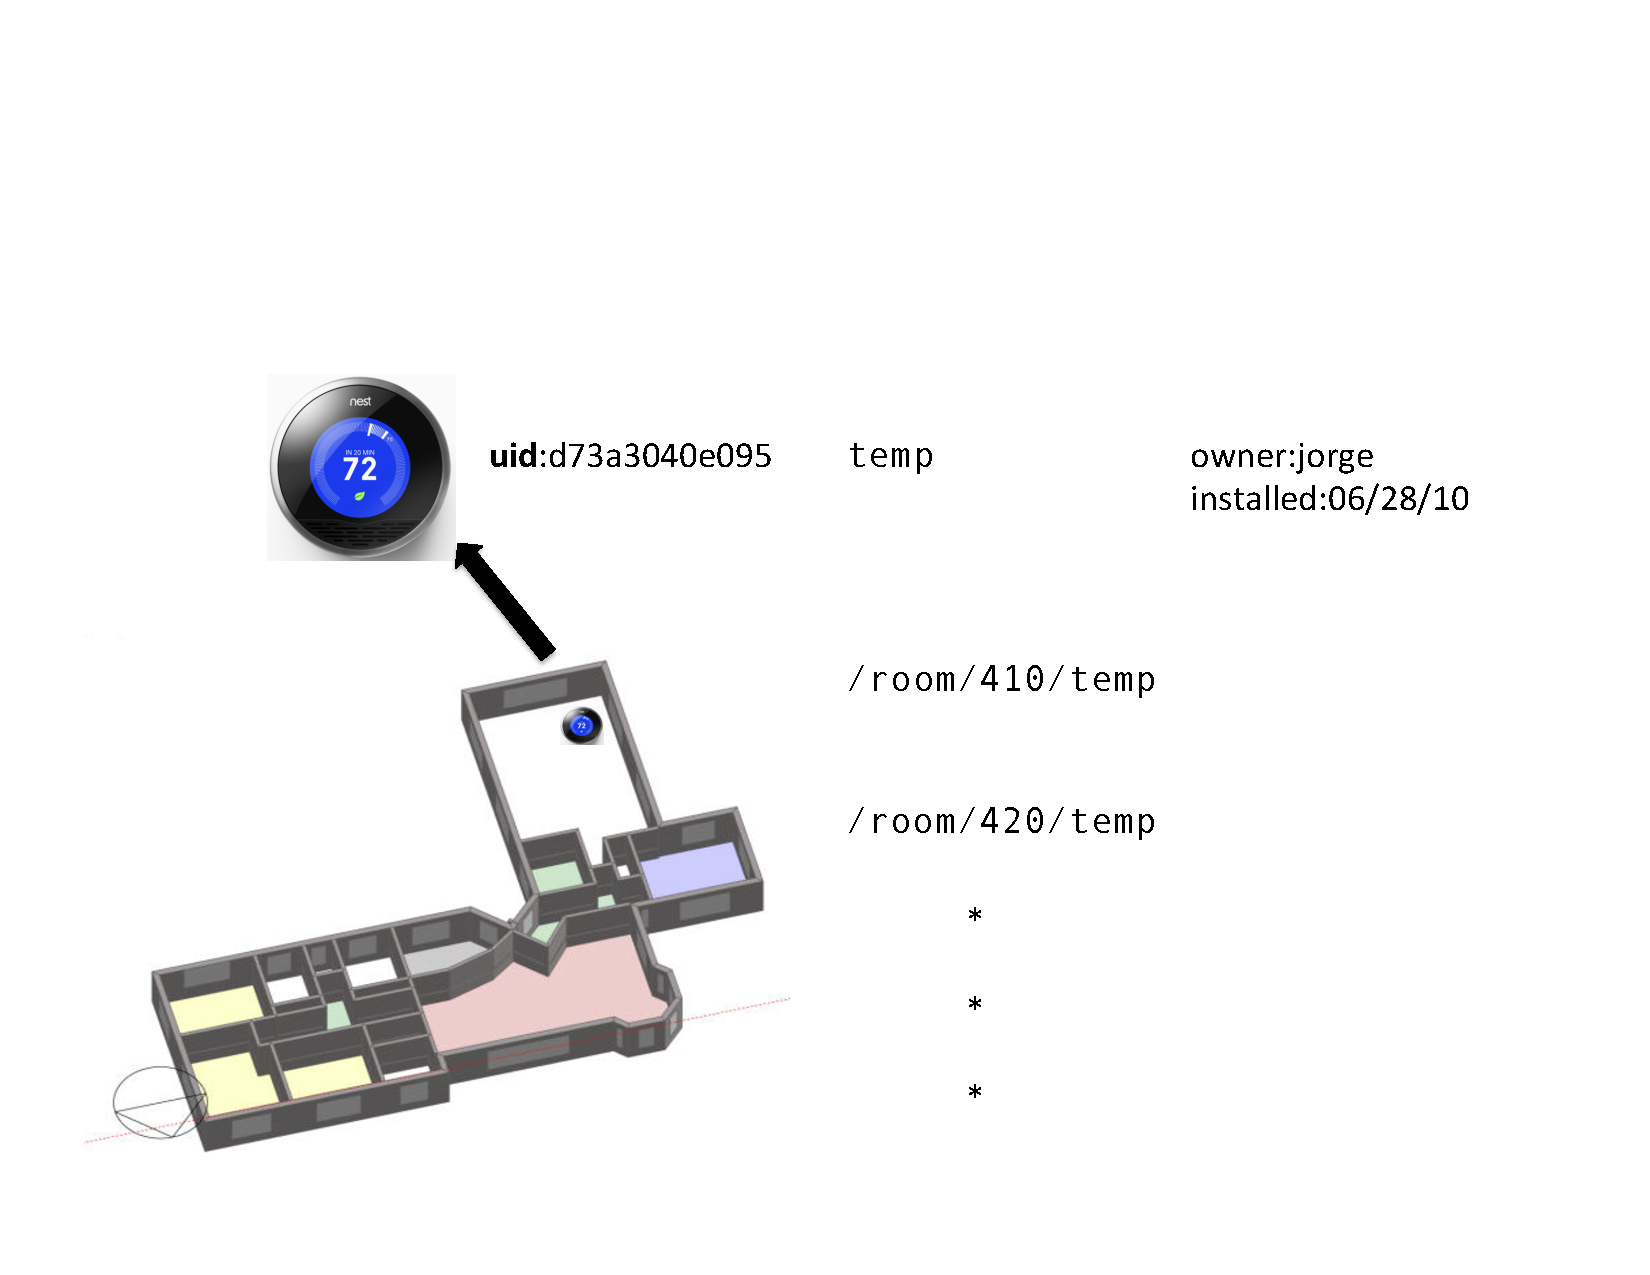
\includegraphics[width=0.65\columnwidth]{figs/everythingfile}
\caption{Everything is a file.  Temperature sensor represented as a file in a folder that contains folders for each room.
Note, the file that represents a temperature sensor producing a stream is given a unique identifer.  The user may also
decorate the file with extra metadata for searching purposes.}
\label{fig:everythingfile}
\end{figure}

In this example, the user is creating a temperature stream file in every room of the building.  The name of the file, given by the user,
is \emph{temp}.  Upon creation, the file is uniquely identified by the system using a unique identifier, as shown.  Like in a unix filesystem, the
file is created within a folder.  Ideally, the name of the folder would encode the placement of the sensor.  In the figure, the 
user is create a temperature stream file in room 410 and room 420.  Note the full filepath for the stream file is /room/410/temp.
During creation, the user may also decorate the file with extra metadata, also shown in the figure.  In this example, they have annotated
the file with information about the owner and when the sensor was installed.   This metadata is used for quickly locating the file
or grouping files that contain similar tags, quickly.

\subsection{File types and operations}
As we map the filesystem abstraction into this problem space, we need to consider the various kinds of files our system will contain,
their semantics, and how our system will expose and manage them.  There are essentially 4 types of files and 6 sub-types.  We summarize
these in Table~\ref{tab:filetypes}.  There are also different kinds of operations that the each file type supports.  Operational semantics
are file dependent.  For example, when you \emph{read} a folder, you obtain the metadata associated with the folder and the name
of its children.  When you \emph{read} a stream, you its metadata and the last timestamp-value it produced.  \emph{Writ}ing to a stream
is a bit different.  You can write to a stream to update its metadata tags and the stream source can write a value to it.  The stream
source is identified with a \emph{publish identifier} (pubid).  The stream source includes the pubid in the write operation for 
the specified stream file.  Without the pubid, the source cannot write to the file.  Any other writer should not be allowed to write to 
a stream file either.  

\begin{table}[h]
\begin{center}
\begin{tabular}{| r | l | l |}
	\hline
	\textbf{type} & \textbf{description} & \textbf{valid operations} \\ \hline
	default/folder & Container file.  Used to group other  & read, write, delete  \\
				   & kinds of files within it.  &  \\ \hline

	stream & Represents a data stream. & read, write, delete, subscribe, \\
			&							&query \\ \hline

	controller & Represents a controller. & read, write, subscribe \\ \hline

	special & There are several kinds of special files for  & read, delete \\
		    & management of jobs and pipes. &  \\ 
	\hline
\end{tabular}
\caption{Summary of the 4 main file types and their valid operations in StreamFS.}
\label{tab:filetypes}
\end{center}
\end{table}

Similar to a traditional filesystem, StreamFS includes \emph{special files}.  There are 6 special files and 5 of them 
are for management purposes.  The only one that is not is the \emph{symbolic link} file, which is essentially used to support
multi-naming and inherents the operational semantics of the file it points to.  The delete operation on a symlink, however,
only deletes the symlink.  A description of these files and the operations they support is given in Table~\ref{tab:filesubtypes}.
A detailed description and examples with be presented in later sections.


\begin{table}[h]
\begin{center}
\begin{tabular}{| r | l | l |}
	\hline
	\textbf{operation} & \textbf{file type} & \textbf{semantics} \\ \hline
	read & folder, stream, ipd, ipi, epd, epi, sub & read the metadata and tags for \\
		 &										   & the associated file. \\ \hline
	write &  stream & Write to stream file, only the \\ 
		  & 		& appropiate stream source is permitted.\\ \hline
	delete & folder, stream, ipd, ipi, epd, epi, sub & Folder must be empty.  \\
		   & 										 & The others can be directly deleted. \\ \hline
	query &  stream, all & streams support time-range queries.  \\
		  &			     & All support metadata-tag queries.\\ \hline
	subscribe & stream & Forwards data from a stream to the\\
			  &		   & specified destination.\\
	\hline
\end{tabular}
\caption{File opertaitons, the file types that support them, and their general semantics.}
\label{tab:semantics}
\end{center}
\end{table}

\subsubsection{Default, Stream, and Controller Files}


\subsubsection{Special Files}

\begin{table}[h]
\begin{center}
\begin{tabular}{| r | l | l |}
	\hline
	\textbf{type} & \textbf{description} & \textbf{valid operations} \\ \hline
	internal process defintion (ipd) & Javascript process definition.  & read, write, delete  \\ \hline

	internal process instance (ipi) & Management file used for managing & read, delete \\
							  & active processing of this script. & \\ \hline

	external process definition (epd) & Gives information about where an & read, write, delete \\
								& external process lives. &\\ \hline

	external process instance (epi) & An active processing stream to an  & read, write, delete \\
								& external process. &\\ \hline

	subscription instance (sub) & An instance of a subscription.  Contains & read, delete \\
								& information about the subscription, &\\
								& such as source/sink and related statistics &\\ \hline
	symbolic link (symlink) & Similar to a symbolic link in Unix. & \\
	\hline
\end{tabular}
\caption{Summary of the 6 special-file sub-types and their valid operations in StreamFS.}
\label{tab:filesubtypes}
\end{center}
\end{table}




\section{Processing Pipelines and Management}
	\subsection{Entity Relationships}

\section{Internal Processes}
Internal processes are jobs submitted to StreamFS that are written in Javascript and managed within a StreamFS cluster.


\section{External Processes}

\subsection{Introduction}
The United States leads the world in per-capita energy consumption.
Our electricity use has consistently increased over the last 40 years~\cite{oecd2011} and other parts of the world are rising all 
too rapidly.  With the specter of climate change and the increasing cost of energy, we must explore new
ways for individuals to gain visibility and insight into their energy consumption in order to optimize and reduce it. 
With the increasing penetration of embedded sensors in the environment and
the continued rise in smartphone adoption, we see an opportunity for smartphones to bridge the physical world
to our computational infrastructure and provide an `energy lens' on the physical world.  

We use mobile phones to construct an entity-relationship 
graph of the physical world and combine it with streaming sensor data in order to perform detailed energy-attribution.
We limit the scope of the world to a single building domain.  We have designed and implemented a real-time, mobile energy auditing
application, called the `Energy Lens', that allows us to collect information about 
things throughout the building and how they are related to each other.  For example, computer X is inside 
room Y and connected to meter Z.  Then, we use these relationships to guide our data look-up and analytical
calculations.  For example, the load curve of room Y consists of the sum of all the power traces for loads
inside room Y.  We use the mobile smartphone as the main input tool.  Our work examines \emph{three main challenges} in setting up and 
deploying a real, whole-building infrastructure to support real-time, 
fined grained energy analytics.  

The first challenge is related to tracking and mobility.
The use of mobile phones presents classical, fundamental challenges related to mobility.  Typically, mobility
refers to the phone, as the person carrying it moves from place to place.  However, in the energy-attribution
context, we are also referring to the movement of energy-consuming objects.  Tracking their relationships to spaces 
and people is as important as tracking people.  We describe how we deal with \emph{both moving people and 
moving objects} and show that these historically difficult problems can be addressed relatively easily, if the proper infrastructure is 
in place.  %We provide evidence that the approach is simple, incrementally deployable, and scalable.

The second challenge is about capturing the inter-relationship semantics and having these inform our  analytics.
We adopt the general notion of physical tags that identify objects in the world.  Our system uses \emph{QR codes} to tag things and locations 
in the physical world.  However, \emph{any tag that provides a unqiue identifier for an object could serve the same purpose}.
Once tagged, there are three types of interactions -- 
registration, linking, and scanning -- which establish important relationships.  Registration is the act of creating a virtual object 
to represent a physical one.  Linking captures the relationship between pairs of objects.  Scanning is the act of performing an item-lookup.
Each of these interactions requires a set of swiping gestures.  Linking requires two tag swipes while the other two actions
require a single tag swipe.  Internally, we maintain a \emph{entity-relationship graph (ERG)} of things, people, and locations, that gets
updated through these sets of gestures.

The third challenge is about indoor network connectivity and access.
In order to connect these components, we rely on having `ubiquitous' network connectivity.  However, in practice, network
\emph{availability} is intermittent and our system must deal with the challenges of intermittency.  We discuss how caching
and logging are used to address these challenges.  Moreover, when connectivity is re-established, we must deal with
applying updates to the ERG, as captured by the phone while disconnected.  
% Conflicts can also occur during an update.  For example, the two updates may disagree about which items are attached
% to which meters.  We implement a very simple conflict resolution scheme, described in section~\ref{sec:conflicts}.
% Finally, certain physical-state transitions are represented as a set of updates to the ERG that must be applied 
% atomically.  We implement transactions in the log-replay and transaction manager.
% Our `Energy Lens' system is deployed in a building on our campus.  We discuss
% its architecture and our design choices.  
  
% We also discuss novel strategies for tracking moving people/things and describe how we implement these in our system.  In summary, our work
% makes the following contributions:

% \begin{itemize}
% \item We design and implement a system that captures and combines physical entities, their inter-relationships, and real-time sensor data 
% 		in buildings.% using mobile phones, qr code, and a cloud-based infrastructure.
% \item We observe that certain combinations of swipes give us useful information to set the location of people and things over time.
% 		We codify this observation in our \emph{context-tracker} and use it to maintain consistency between the entity-relationship graph and the 
% 		state of the physical world.  To the best of our knowledge, this is radically different from the approaches in standard 
% 		localization techniques.  However, we argue that it can be used to \emph{enhance} their accuracy and overall performance.
% \item We implement a prefetching algorithm to obtain context-dependent information to both improve performance and
% 		enable disconnected operation.  We also design and implement a log-replay and transaction manager over our data management layer.  We describe how different conflict-resolution policies can be implemented and our rationale for the policies we chose.
% \end{itemize}

% \vspace{0.08in}

% In the next sections we go through a motivating scenario.  We then discuss some related work, followed 
% by the system architecture, evaluation, and future directions.

\section{Process Management}
%\input{external_tex/streamfs_aggregation/}
Sensor data is fundamentally challenging to deal with because much of it must be cleaned before it can be processed.  For example,
it is not uncommon to receive readings that is out of operational range, that is erroneous with respect to the previous observed trend,
or to stop receiving readings altogether.  This implies the need for processing jobs to provide a level of filtering over the raw streams.
Once the data is cleaned, it is typically consumed more sophisticated processes that aggregate the information or use it for control
of the space or equipment.  We provide the mechanisms for handling both classes of processing jobs with our process management layer.
In the next section we will discuss our process management layer and how users can both submit jobs to StreamFS for management or link
their own external processing elements so that they can be managed through StreamFS but run outside of StreamFS.


\section{Mapping OLAP to ERG}

\begin{itemize}
\item Introduction to OLAP.
\item Explanation of ERG in StreamFS.
\end{itemize}
Online analytical processing (OLAP) is a processing layer that provides summurization of data
from a set of underlying data repository (date warehouses).  Traditionally, OLAP is used to process
business data.  Business data summurization allows an analyst ask targetted questions about aggregates 
and trends in their data.  The data is typically multidimensional in nature and operations can be performed with
respect to those dimensions and their inter-relationship.

\subsection{Measures, Dimenions, and Levels}

\subsection{Operations: drill-down and roll-up}

\subsection{Operations: slice and dice}

\subsection{Operations: pivoting}
\section{Dynamic Aggregation}
\label{sec:dynagg}
Dynamic aggregation combines the underlying entity-relationship graph with in-network aggregation.  It treats
each node in the graph as a potential point of aggregation on a particular data type.  For example,
if we need to compute aggregates of \emph{KW} data and we declare the node for a particular room as
the point of aggregation, we accept data from all children of that node that, whose units are in \emph{KW},
and add the streams together over pre-defined window size or pre-defined timeouts.

The scheme is hiearchical, so a node only accepts data from its children and only sends data to its parent.
StreamFS checks for cycles when before node insertion and prevents double-counting errors by only allowing 
aggregation-points that are roots of a tree that is a sub-graph of the entity-relationship graph.  In our deployment,
each view is a managed as an independent hierarchy.  So the hierarchy of \emph{spaces} is separate from
the \emph{inventory} hierarchy or the \emph{taxonomy} hierarchy.  This allows us to ask questions with a particular
view in mind, without conflict, and is a natural fit for our aggregation scheme.

\subsection{How it works}
Although there are different semantics applied to different node types at the application layer, StreamFS only knows
about two types of nodes: (1) default nodes and (2) stream nodes.  The main difference is that \emph{default} nodes
are not explicitly associated with data coming from a sensor and \emph{stream} nodes are.  Furthermore, default
nodes can have children, while stream nodes cannot.  In our application, meters are represented by default nodes
and each stream of data they produce is a stream node.

When an aggregation point is chosen and enabled, dynamic aggregation places a buffer at the node for the type
of data that should be aggregated.  If we want to aggregate \emph{KW} data, we specify the type and send an enable-aggregation
request to the node through an HTTP {\texttt POST} to the path for that node.  The flow of data starts at the leaves when
a stream node received data from a sensor through HTTP {\texttt POST}.  As data arrives it is immediately
forwarded upstream to the parent(s).  If a node that receives data from its children is an aggregation point it buffers
the data, otherwise it fowards it to its parent.

Ignoring the timeouts for now, lets imagine the parent is a point of aggregation and its buffer is full.  At this point
the parent separates data into bins for each source and cleans it for aggregation through interpolation.  The main
operation is to \emph{stretch} and \emph{fill} that data with linearly interpolated values.  The \emph{stretch}
operation orders all the timestamps in increasing order and for each bin (signal) interpolates the values using the
first (last) pair of data points.  If there is only a single data point, the stretch uses it as the missing value.
The \emph{fill} operation find the nearest timestamps that are less-than and greater-than the missing sampling time, 
uses their values to determine the equation of a line between them and interpolates the missing value using that equation.
Once this is done for each signal, the values are added together for each unqiue timestamp and the aggregated
signal is reported to the parent, where the operation occurs recursively to the root.
Figure~\ref{fig:aggtree} shows an illustration of its operation.  

%problem:  the buffer size has to increase exponentially up the tree, in order to not drop any values.
%solution: chuck the data into default-buffer sized pieces and parallelize the interpolation using the interpolated tasks technique


%FILL IN WITH REAL GRAPH
\begin{figure}[htb!]
\begin{center}
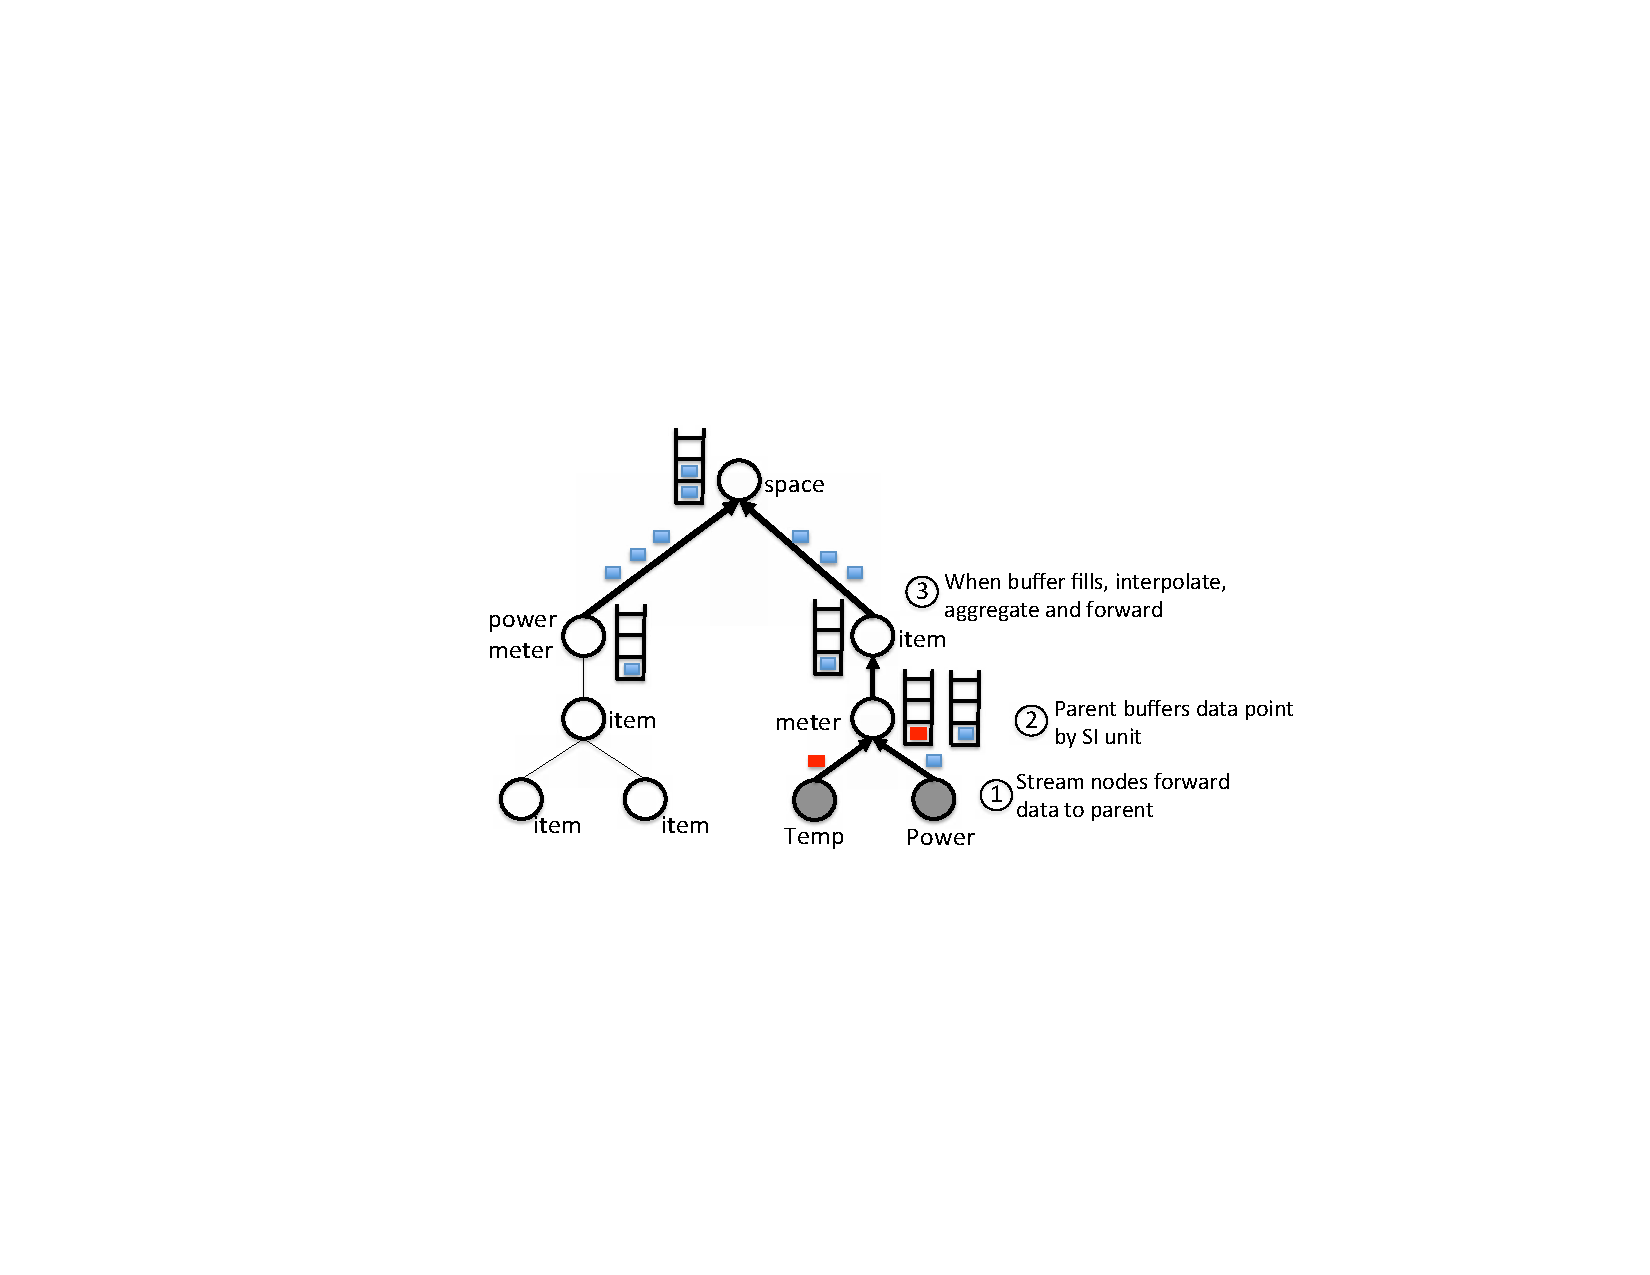
\includegraphics[scale=0.6]{figs/aggtree}
\caption{This shows an illustration of the aggregation tree used by \emph{dynamic aggregation}.  Data flows from 
the leaves to the root through user-specified aggregation points.  When the local buffer is full the streams
are separated by source, interpolated, and summed.  The aggregated signal is foward up the tree.}
\label{fig:aggtree}
\end{center}
\end{figure}

\subsubsection{Dealing with dynamics}
This approach deals with changes in the graph quite naturally.  All aggregation point deal only with local data, so
a node is only concerned about the children that give it data and the parent to send data to.  As objects in the environment
move from place to place and these changes are captured, the entity-relationship graph also changes to reflect the move.
This change in aggregation constituents is naturally accounted for in the aggregate.  If a child is removed,
it no longer forwards data to the old parent, therefore the aggregate will reflect that change.
Note, however, that changes in the entity-relationship graph are indistinguishable from energy-consuming items that have
been turned off.  For the purposes of aggregation, that is okay.

\subsubsection{Two scenarios}
We illustrate dynamic aggregation with a common usage scenario.  Imagine there are a number of people in a building,
each owning a number of plug-load applicances and a laptop.  Assume that when a person is in a room their laptop
is plugged in and when they leave the room they unplug their laptop and take it with them.  People come and go
throughout the day, changing the aggregate power consumption of the room and it happens.  In addition, some
of those people move to other rooms and plug their laptop in the new location.  As this happens, we will assume
all actions are being recorded in StreamFS.

%FILL IN WITH REAL GRAPH
\begin{figure}[htb!]
\begin{center}
\subfloat[Room 1 object and aggregate streams.]{%
            \label{fig:dynaggs1room1}
            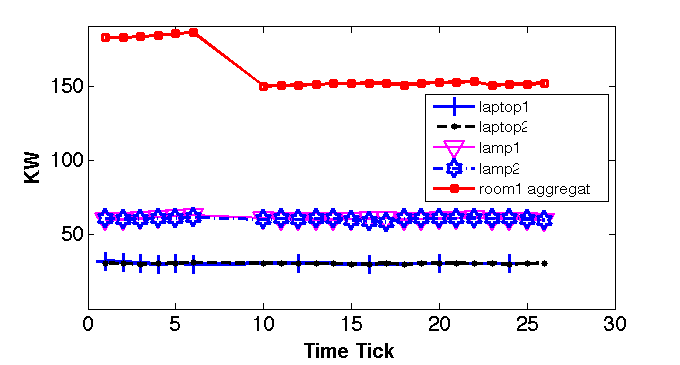
\includegraphics[scale=0.4]{figs/dynagg_scenario1_room1}
        }
\subfloat[Room 2 aggregate.]{%
            \label{fig:dynaggs1room2}
            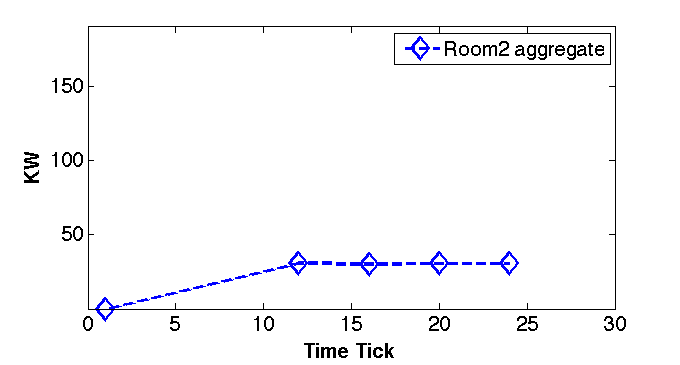
\includegraphics[scale=0.4]{figs/dynagg_scenario1_room2}
        }
\end{center}
\caption{
	The power consumes by a laptop in \emph{room 1} is shifted to \emph{room 2} a time t=7.  Notice the aggregagate drops in room 1
	while it rises in room 2.
     }%
\label{fig:multiroomagg}
\end{figure}

Figure~\ref{fig:multiroomagg} illustrate the aggregation results of that scenario.  Notice how...

% For demonstration lets have the user turn off on of their appliances when they leave as well.  This should cause that total
% room aggregate to drop, the person's personal aggregate to drop, but the other occupant's aggregate to remain
% the same.

% %FILL IN WITH REAL GRAPH
% \begin{figure}[htb!]
% \begin{center}
% 
\includegraphics[scale=0.39]{figs/blankbox}
% \caption{A room with items that belong to many users.  Person leaves with their item, aggregate falls.  Show aggregate.
% Person joins another room, aggregate in that room rises.  Show aggregate in the new room.  Compare before and after.}
% \label{fig:personaltotalagg}
% \end{center}
% \end{figure}

% Figure~\ref{fig:personaltotalagg} illustrate the results of the second sceanrio.  Note how...



\section{API Overview}
	\subsection{RESTful API}
	\subsection{Programmatic API}
\section{Example Application: Deployment Viewer}
\section{Example Application: Mounted Filesystem and Matlab Integration}
\section{Summary}




